% vim:autoindent:set textwidth=78:

\section{Working with Projections}\label{label_projections}
\index{Projections!working with}

% when the revision of a section has been finalized, 
% comment out the following line:
%\updatedisclaimer

QGIS supports on-the-fly (OTF) projection of vector layers. This feature allows you
to display layers with different coordinate systems and have them overlay
properly.

\subsection{Overview of Projection Support}\label{label_projoverview}

QGIS has support for approximately 2,700 known projections. 
Projections are stored in a SQLite database that is installed with QGIS.
%Appendix \ref{app:datamodel}  contains information about the database and the
% schema. 
Normally you do not need to manipulate the database directly. In fact,
doing so may cause projection support to fail. Custom projections are
stored in a user database. See Section \ref{sec:customprojections} for
information on managing your custom projections.

The projections available in QGIS are based on those defined by
EPSG\index{EPSG} and are largely abstracted from the spatial\_references 
table in PostGIS\index{PostGIS} version 1.x. The EPSG identifiers are
present in the database and can be used to specify a projection in QGIS.

In order to use OTF projection, your data must contain information about its
coordinate system. For PostGIS layers QGIS uses the spatial reference
identifier that was specified when the layer was created. For data supported
by OGR, QGIS relies on the presence of a format specific means of specifying
the coordinate system. In the case of shapefiles, this means a file containing
the Well Known Text (WKT)\index{WKT} specification of the coordinate
system. The
projection file has the same base name as the shapefile and a prj extension.
For example, a shapefile named \filename{alaska.shp} would have a 
corresponding projection file named \filename{alaska.prj}.

%\section{Requirements}
%QGIS uses the Proj4 to provide projection support. 

\subsection{Getting Started}\label{label_projstart}

At startup, QGIS does not have OTF projection enabled. To use OTF
projection, you must open the \dropmenuopttwo{mActionOptions}{Project Properties} dialog, select a
projection for the map and enable OTF projections. There are two ways to open
the \dialog{Project Properties} dialog:

\begin{enumerate}
\item Select \dropmenuopttwo{mActionOptions}{Project Properties} from the \mainmenuopt{Settings} menu.
\item Click on the \toolbtntwo{mIconProjectionEnabled}{projector} icon in the lower right-hand corner of the
statusbar.
\end{enumerate}

The Projection tab of the \dialog{Project Properties} dialog contains four important components as numbered in Figure
\ref{fig:projections} and described below.

\begin{figure}[ht]
   \begin{center}
   \caption{Projection Dialog \nixcaption}\label{fig:projections}\smallskip
   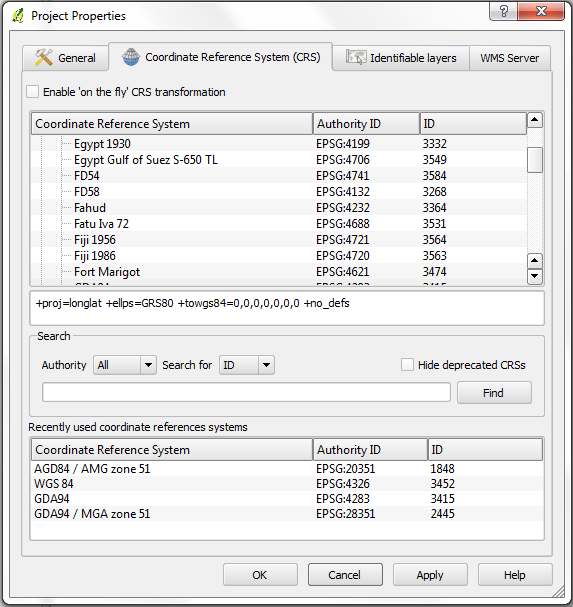
\includegraphics[clip=true, width=14cm]{projectionDialog}
\end{center}  
\end{figure}

\begin{enumerate}
\item \textbf{Enable on the fly projection}\index{Projections!enabling} - this checkbox is used
to enable or disable OTF
projection. When off, no projection takes place and each layer
is drawn using the coordinates as read from the data source. When on, the
coordinates in each layer are projected to the coordinate system of the map
canvas.
\item \textbf{Projections} - this is a list of all projection supported by QGIS,
including Geographic, Projected and Custom coordinate systems. To use a
coordinate system, select it from the list by expanding the appropriate node
and selecting the projection. The active projection is pre-selected.
\item \textbf{Proj4 text} - this is the projection string used by the Proj4 projection
engine. This text is read-only and provided for informational purposes.
\item \textbf{Search} - if you know the EPSG identifier or the name 
for a projection, you can use the search feature to find it. Enter the 
identifier and click on \button{Find}.
\end{enumerate}

\begin{Tip}
 \caption{\textsc{Project Properties Dialog}}
\qgistip{
If you open the \dialog{Project Properties} dialog from the \mainmenuopt{Settings} menu, you
must
click on the \tab{Projection} tab to view the projection settings. Opening
the dialog from the \toolbtntwo{mIconProjectionEnabled}{projector} icon will automatically bring the
\tab{Projection} tab to the front.
}
\end{Tip}

\subsubsection{Specifying a Projection}
\index{Projections!specifying}
\label{sec:projection-specifying}

QGIS automatically sets the map projection to the coordinate system of the
first layer loaded. One way to specify the map projection is to first load a
layer with the projection you want for the entire map. Then open the
\dialog{Project Properties} dialog and click on the \checkbox{Enable on the fly
projection} checkbox. You can now close the \dialog{Project Properties} dialog
and add additional layers to the map. 

If you have already added layers and want to enable OTF projection, open the 
\tab{Projection} tab of the \dialog{Project Properties} dialog and find the projection or geographic
coordinate system you want to use in the list of projections. Alternatively
you can use the search feature as described in the previous section.

\subsection{Custom Projections}\label{sec:customprojections}
\index{Projections!custom}

If QGIS doesn't have the projection you need, you can define a custom
projection. To define a projection, select \dropmenuopttwo{mIconNew}{Custom CRS} from
the \mainmenuopt{Settings} menu. Custom projections are stored in your QGIS user
database. In addition to your projections, this database contains your spatial
bookmarks and other custom data. 

\begin{figure}[ht]
   \begin{center}
   \caption{Custom Projection Dialog \nixcaption}\label{fig:customprojections}\smallskip
   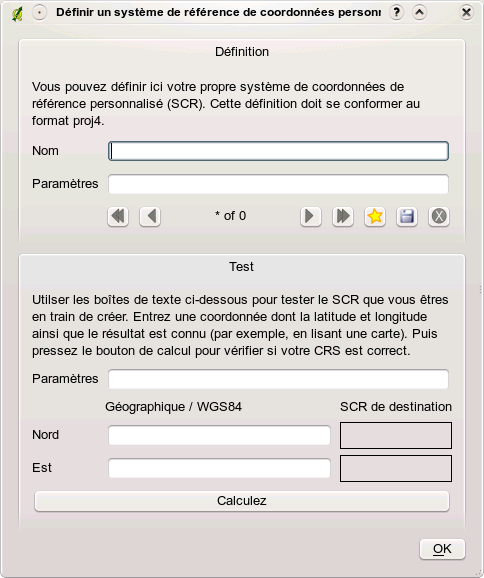
\includegraphics[clip=true, width=14cm]{customProjectionDialog}
\end{center}  
\end{figure}

At version \CURRENT of QGIS, defining a custom projection requires a good
understanding of the Proj.4 projection library. To begin, refer to the
Cartographic Projection Procedures for the UNIX Environment - A User's Manual
by Gerald I. Evenden, U.S. Geological Survey Open-File Report 90-284, 1990
(available at \url{ftp://ftp.remotesensing.org/proj/OF90-284.pdf}).
This manual describes the use of the \usertext{proj.4} and related command line
utilities. The cartographic parameters used with \usertext{proj.4} and described
in the user manual are the same as those used by QGIS. 

The \dialog{Custom Coordinate Reference System Definition} dialog requires
only two parameters to define a user projection: 
\begin{enumerate}
\item a descriptive name and
\item the cartographic parameters in PROJ.4 format.
\end{enumerate}
To create a new projection, click the 
\toolbtntwo{mIconNew}{New} button and enter a descriptive
name and the projection parameters. 
After that you can save your projektion by clicking the button
\toolbtntwo{mActionFileSave}{Save}.

Note that the \guilabel{Parameters} must begin with a \usertext{+proj=}-block,
to represent the new projection.

Figure \ref{fig:customprojections} shows
the dialog with an example projection. The parameters shown were entered based
on a knowledge of the projection and the information found in OF90-284.

You can test your projection parameters to see if they give sane results by
clicking on the \button{Calculate} button inside the \guiheading{Test} block 
and pasting your projection parameters into
the \guilabel{Parameters} field. Then enter known WGS 84 latitude and longitude
values in \guilabel{North} and \guilabel{East} fields respectively. 
Click on \button{Calculate} and compare the results with the known values in your projected coordinate
system. 

